%%
%% $Id$
%%
%% Copyright (c) 2007-2008 Christian Fehler
%% Copyright (c) 2007-2008 Benjamin Mies
%%


%### removes texlipse warnings


\chapter{Oberfläche}\label{GUI}

In diesem Kapitel geht es um die Oberflächengestaltung. Zum Einen geht es darum,
wie und warum die Hauptansicht so gestaltet wurde, zum Anderen darum, welche
besonderen Schritte notwendig waren, um das Aussehen zu verbessern, und es dem
Benutzer dadurch zu erleichtern, mit dem \gtitool zu arbeiten.\vspace{10pt}


\section{Gestaltung der Hauptansicht}\label{GUIMain}

Als wir zu Beginn der Diplomarbeit über die Gestaltung der Hauptansicht
diskutiert haben, kamen wir sehr schnell zu der Übereinkunft, dass die
Ähnlichkeit zu dem Lernwerkzeug TPML, siehe \cite{tpml}, möglichst groß sein
sollte. Da sowohl "`Grundlagen der theoretischen Informatik"', als auch "`Theorie der
Programmierung I"' für jeden Informatikstudenten der Universität Siegen
Pflichtveranstaltungen sind, ist die Wahrscheinlichkeit, dass Studenten beide
Lernwerkzeuge nutzen werden, sehr hoch.\vspace{10pt}

Ein großer Vorteil dieser Entscheidung war natürlich, dass wir beide
bereits an der Projektgruppe TPML mitgearbeitet hatten. Zwar waren wir nicht
hauptsächlich an den Grafikelementen beteiligt, konnten aber dennoch einige
Einblicke sammeln, welche uns bei der Gestaltung der Benutzeroberfläche sehr
geholfen haben. Wir hoffen, dass zukünftige Benutzer von den Parallelen im Aussehen
und in der Funktionsweise beider Lernwerkzeuge profitieren können.\vspace{10pt}

Während der gesamten Diplomarbeit stand im Vordergrund, das Lernwerkzeug so
intuitiv und selbsterklärend wie möglich zu gestalten. Denn schließlich soll
ein Benutzer nicht noch lange Zeit darauf verwenden müssen, den Umgang mit dem
Werkzeug zu erlernen.\vspace{10pt}

Aus diesem Ansatz heraus ist zum Beispiel auch der Wizard zum Anlegen einer
neuen Datei enstanden. Dieser Wizard hat für jedes Eingabefeld einen
Vorschlag, welche in den Einstellungen auf die Benutzerwünsche angepasst werden
kann. Beim ersten Start sollen diese Werte als Orientierung dienen, was in den
Feldern eingetragen werden muss.
\vspace{10pt}


\section{Gestaltung der graphischen Komponenten}\label{GUIDesign}

Wir wurden an einigen Stellen im \gtitool vor das Problem gestellt, Algorithmen
schrittweise ablaufen zu lassen, da der Benutzer bei der Unterteilung in kleine
Schritte mehr Nutzen hat, als wenn der Algorithmus in einem Schritt abgearbeitet würde.
Wir entschieden uns dafür, eine Navigationsleiste zu verwenden, die es dem
Benutzer gestattet, in dem Algorithmus einen Schritt vor bzw. einen Schritt
zurück zu gehen. Um die Handhabung für den Benutzer zu erleichtern, wurde die
Navigationsleiste so erweitert, dass der Benutzer sowohl zurück an den Anfang der
Ausführung des Algorithmus springen kann, als auch an das Ende. Des weiteren
können die einzelnen Schritte auch automatisch, nach einer einstellbaren Zeit,
durchgeführt werden.\vspace{10pt}

In vielen Ansichten werden neben der Hauptansicht Tabellen angezeigt. In
diesen Tabellen werden zusätzliche Informationen aufgelistet,
welche oft mit Übergängen oder Zuständen verknüpft sind. Klickt man
eine Spalte aus der Tabelle an, werden die zugehörigen graphischen
Komponenten farblich hervorgehoben. Diese Funktion ist zum Beispiel
bei der Fehlertabelle sehr hilfreich, da man die betroffenen
Stellen in dem Automaten oder der Grammatik schneller lokalisieren
kann.\vspace{10pt}

Eine weitere Anpassung, die von uns implementiert wurde, ist die  Verwendung von
sogenannten {\em Pretty-Strings}. Ein Pretty-String unterscheidet sich von einem
normalen String durch zu\-sätz\-liche Farbinformationen und Zeichenattribute
jedes einzelnen Zeichens. Der Benutzer soll dadurch in der Lage sein, die ihm
zur Verfügung gestellten Informationen schneller aufzunehmen, als wenn ihm eine
unformatierte Zeichenkette angezeigt werden würde.\vspace{10pt}


\section{Anpassung aller GUI Komponenten}\label{GUIAdaption}

Ein wichtiges Konzept bei der graphischen Gestaltung des \gtitool ist es, die von
der Programmiersprache zur Verfügung gestellten Komponenten anzupassen und dann
nur noch ausschließlich diese angepassten Komponenten zu benutzen. Der Vorteil
dieser Umsetzung ist, dass nicht überall ein normaler String verwendet wird,
sondern der in Abschnitt \ref{GUIDesign} angesprochene Pretty-String. Ein
weiterer Vorteil dieser Umsetzung ist, dass Anpassungen der Oberfläche immer sehr
schnell gemacht werden können, da nur jeweils eine Komponente angepasst werden
muss.\vspace{10pt}

Der erforderliche Aufwand wurde investiert, um dem Benutzer eine möglichst
ansprechende Oberfläche zu präsentieren und ihn durch die zusätzlichen
Informationen zu unterstützen, die Inhalte besser zu verstehen.\vspace{10pt}

Ein weiterer wichtiger Ansatz war, dass der Benutzer das \gtitool möglichst
intuitiv bedienen kann. Zur Umsetzung wurde unter anderem Drag and Drop auf den
verschiedenen Komponenten implementiert. So kann der Benutzer im Übergangs-Dialog
die Symbole einfach vom "`Alphabet"' in die "`Übergangs-Menge"' ziehen. Gleiches
gilt für das Umsortieren von Produktionen, wodurch zwar die Grammatik nicht
geändert wird, es dem Benutzer aber möglich ist, die Produktionen übersichtlicher
anzuordnen. In vielen Programmen, in denen Tabs zur Gliederung benutzt werden,
gehört es zum Funktionsumfang diese Tabs per Drag and Drop zu verschieben. Auch
dies wurde implementiert, um dem Benutzer die Möglichkeit zu geben, seine Daten besser zu
organisieren.\vspace{10pt}


\section{Look \& Feel}\label{LookAndFeel}

Damit das \gtitool unter verschiedenen Betriebsystemen immer gleich, oder
zumindest sehr ähnlich aussieht, kam während der Entwicklung der Wunsch auf, ein
eigenes Look \& Feel zu verwenden. Java bietet in diesem Bereich zwar mit dem
Metal Look \& Feel eine Lösung an, die unter allen Betriebssystemen gleich
aussehen soll. Diese erfüllte aber unsere Vorstellungen nicht. Schließlich fiel
die Wahl auf TinyLaF (siehe \cite{tinylaf}). Dem Benutzer ist es aber
freigestellt, ein anderes, zum Beispiel das normale Betriebsystem Look \& Feel zu
verwenden, wenn er dies wünscht. Alle in dieser Diplomarbeit verwendeten Bilder
des \gtitools wurden mit TinyLaF als Look \& Feel erstellt.\vspace{10pt}


\section{Zweite Ansicht}\label{SecondView}

Bei der Umsetzung der verschiedenen Algorithmen wurden wir vor das Problem
gestellt, dass es sinnvoll wäre, einen Automaten nach der Umwandlung, mit dem
Automaten oder der Grammatik vor der Umwandlung zu vergleichen. Dies war nur
durch einen Tabwechsel oder das Öffnen eines zweiten \gtitools möglich, was
nicht besonders benutzerfreundlich ist.\vspace{10pt}

\begin{figure}[h!]
\begin{center}
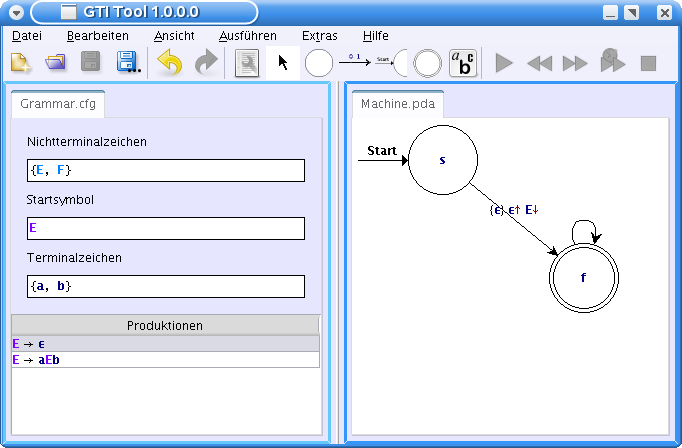
\includegraphics[width=12cm]{../images/second_view.png}
\caption{Zweite Ansicht}
\label{FigureSecondView}
\end{center}
\end{figure}
\vspace{10pt}

Dieses Problem wurde dadurch gelöst, dass eine zweite Ansicht integriert wurde,
die es erlaubt, Tabs in einem zweiten Bereich zu öffnen. So können zwei Dateien
gleichzeitig sichtbar sein. Während der Umsetzung mussten verschiedene Probleme
diskutiert und gelöst werden. So stellte sich die Frage, wie dem Benutzer
verdeutlicht werden kann, welche der beiden sichtbaren Dateien aktiv ist. Wichtig
ist dieser Status für die Aktivierung der Menüeinträge bzw. Toolbar Buttons. Die
Lösung besteht jetzt darin, dass anhand von unterschiedlichen Umrandungen dem
Benutzer klar gemacht werden soll, welche der beiden Dateien aktiv ist. Durch
dieses Vorgehen wird intuitiv klar, welche Datei aktiv ist, da sich die Farbe der
Umrandung beim Aktivieren der anderen Ansicht ändert. In Abbildung
\ref{FigureSecondView} ist der Automat auf der rechten Seite aktiv.\vspace{10pt}

Eine weitere wichtige Eigenschaft der zweiten Ansicht ist, dass Dateien in diese
zweite Ansicht verschoben werden können. Ebenfalls ist es möglich, in der zweiten
Ansicht Dateien zu öffnen bzw. neue zu erstellen. Um die letzten beiden genannten
Punkte umzusetzen, wurde das Konzept des aktiven Editors erweitert. Die oben
beschriebene andere Darstellung der aktiven Datei wurde so erweitert, dass sich
auch alle anderen Ereignisse auf den aktiven Editor beziehen. Wenn eine Datei
geöfffnet werden soll, muss erst die Ansicht aktiviert werden, in der die Datei
geöffnet werden soll. Das Gleiche gilt beim Anlegen einer neuen Datei. Das
Verschieben von geöffneten Dateien wurde per Kontextmenü und per Drag and Drop
zwischen den Ansichten gelöst.\vspace{10pt}


\section{Parser}\label{Parser}

Wenn wir in dieser Diplomarbeit den Begriff {\em Parser} verwenden, meinen wir
damit die Umwandlung einer vom Benutzer eingegebene Zeichenkette in ein internes
Format, das wir benutzen können, um die Daten weiter zu verwenden. Ein Beispiel
dafür ist das Alphabet oder der Zustand. Ein Parser wird normalerweise als Teil
eines Compilers benutzt. Die bei einem Compiler verwendeteten Phasen nach dem
Parsen werden bis auf das Prüfen der kontextsensitiven Bedingungen nicht
benötigt, da keine Umwandlung in eine andere Programmiersprache erfolgen
muss.\vspace{10pt}

\begin{figure}[h!]
\begin{center}
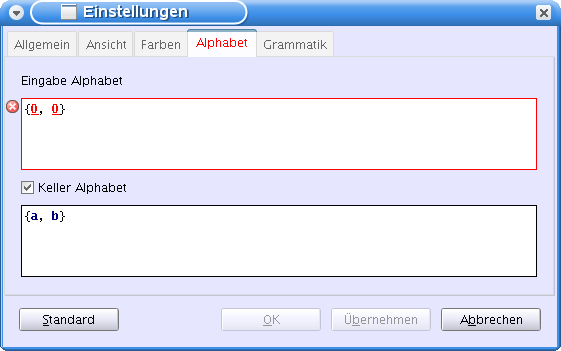
\includegraphics[width=12cm]{../images/parser.png}
\caption{Kontextsensitive Bedingungen}
\label{FigureParser}
\end{center}
\end{figure}
\vspace{10pt}

Zu Beginn der Planungen für das \gtitool stellte sich die Frage, wie der Benutzer
die unterschiedlichen Eingaben machen soll. Es wurden verschiedene
Möglichkeiten in Betracht gezogen, schließlich wurde aber die Verwendung von
Parsern bevorzugt. Der Vorteil von Parsern ist, dass der Benutzer in seinen
Eingaben, für zum Beispiel ein Alphabet, so wenig wie möglich beschränkt wird.
Dies wäre nicht der Fall gewesen, wenn nur eine Auswahl von Zeichen zur
Verfügung gestanden hätte.\vspace{10pt}

Zur Erzeugung der Parser wurde der CUP Parser-Generator für Java verwendet, siehe
\cite{java-cup}. Als Scannergenerator wurde wegen des guten Zusammenspiels mit
dem verwendeten Parser-Generator JFlex benutzt, siehe
\cite{jflex}.\vspace{10pt}

In diesem Abschnitt werden die Besonderheiten der Parser angesprochen, vor allem
das Prüfen der kontextsensitiven Bedingungen und das Anpassen der verwendeten
Darstellungsweise. Desweiteren müssen auch Bedingungen geprüft werden, die im
Zusammenhang mit dem verwendeten Automaten bzw. der Grammatik
stehen.\vspace{10pt}

Wird eine solche Bedingung verletzt, kann der Benutzer geöffnete Dialoge, wie zum
Beispiel den Dialog zum Ändern des Alphabets, nicht mehr bestätigen und ist
gezwungen, den Fehler zu beheben, oder die Bearbeitung abzubrechen. Es besteht
also kein Unterschied zwischen der Behandlung eines Fehlers im Scanner, Parser
oder den kontextsensitiven Bedingungen.\vspace{10pt}


\subsection{Kontextsensitive Bedingungen}\label{ParserContext}

In diesem Abschnitt geht es darum, welche kontextsensitiven Bedingungen
über\-prüft werden müssen, um dem Benutzer zu verdeutlichen, welche Eingaben im
aktuellen Kontext nicht vorgenommen werden können. Ein wichtiger Aspekt dabei
ist, dass der Benutzer darauf hingewiesen wird, warum seine Eingabe abgelehnt
wird.\vspace{10pt}

Im \gtitool gibt es an verschiedenen Stellen die Möglichkeit, ein Alphabet
einzugeben. Betrachten wir als erstes die Eingabe des Alphabetes im Dialog für
die Einstellungen, da dieser Parser die wenigsten kontextsensitiven Bedingungen
berücksichtigen muss. Sowohl beim Eingabealphabet, wie auch beim Kelleralphabet
ist die einzige Bedingung, dass ein Symbol nicht doppelt vorkommen darf, eine
Eingabe \{\Symbol{0}, \Symbol{0}\} wie in Abbildung \ref{FigureParser}
dargestellt, ist somit nicht zulässig.\vspace{10pt}

Ebenfalls in den Einstellungen zu finden ist die Eingabe der
Nichtterminalzeichen, Terminalzeichen und des Startsymbols. Genau wie beim
Alphabet, darf auch hier ein Nichtterminalzeichen bzw. ein Terminalzeichen nur
einmal in der Menge vorkommen. Zusätzlich muss aber gelten, dass die Menge der
Nichtterminalzeichen  und die Menge der Terminalzeichen disjunkt sind. Es
ist dem Benutzer somit nicht erlaubt bei den Nichtterminalzeichen
\{\NonterminalSymbol{E}, \NonterminalSymbol{a}\} und gleichzeitig
\{\TerminalSymbol{a}, \TerminalSymbol{b}\} bei den Terminalzeichen einzutragen.
Versucht der Benutzer eine solche Eingabe vorzunehmen, bekommt er zum Beispiel
bei den Nichtterminalzeichen angezeigt, dass \NonterminalSymbol{a} bereits ein
Terminalzeichen ist, bzw. umgekehrt, wenn zuerst das Nichtterminalzeichen
vorhanden war. Eine weitere Bedingung ist, dass das Startsymbol in der Menge der
Nichtterminalzeichen enthalten sein muss. Auch diese Bedingung wird überprüft
und bei Verletzung eine Fehlermeldung angezeigt.\vspace{10pt}

Eine weitere Kontextbedingung wird überprüft, wenn das Alphabet eines
bestehenden Automaten bearbeitet wird. Dabei darf der Benutzer beliebige, 
noch nicht verwendete Symbole ergänzen. Er darf allerdings keine Symbole
entfernen, die noch von einem Übergang verwendet werden. Soll dies geschehen,
muss der Benutzer erst das Symbol aus allen Übergängen entfernen,
anschließend kann es aus dem Alphabet entfernt werden.\vspace{10pt}

Gleiches gilt für das Bearbeiten der Nichtterminalzeichen und Terminalzeichen
einer bestehenden Grammatik. Auch hier wird überprüft, ob das Zeichen in einer
der Produktionen benutzt wird. Ist dies der Fall, kann es nicht entfernt
werden.\vspace{10pt}


\subsection{Anpassung der Darstellungsweise}\label{ParserAdaption}

Um das Arbeiten mit Grammatiken einfacher und übersichtlicher zu machen, wurde
die Darstellung der Nichtterminalzeichen, Terminalzeichen und des Startsymbols
unterschiedlich gewählt. So werden das Startsymbol und die anderen
Nichtterminalzeichen in einer unterschiedlichen Farbe dargestellt. Der Benutzer
ist somit in der Lage, in den Produktionen zu erkennen, ob ein
Nichtterminalzeichen das Startsymbol ist oder nicht.\vspace{10pt}


\section{Drucken}\label{Print}

Da dieses Lernwerkzeug auch beim Lösen und Nachvollziehen der Übungen
Verwendung finden soll, fanden wir es sehr nützlich und wichtig, dass der
Benutzer seine Lösungen auch ausdrucken kann. Sei es, um diese bei der
Besprechung der Übung zu vergleichen, oder die Ergebnisse auf dem Papier
nochmal nachzuvollziehen.\vspace{10pt}

Daher sind alle Tabellen, welche bei den verschiedenen Funktionen des
Lernwerkzeugs dargestellt werden, druckbar. Weiterhin kann auch der konstruierte
Automat gedruckt werden. Zusätzlich können noch alle Zwischenansichten der
Automaten gedruckt werden, sprich die einzelnen Schritte bei der Konvertierung
oder der Minimierung.\vspace{10pt}

Desweiteren kann ein konstruierter Automat als Bild exportiert werden. So hat
man die Möglichkeit einen Automaten in ein PDF- oder eine \LaTeX -Datei
einzubinden.\vspace{10pt}


%### removes texlipse warnings
